\documentclass{article}
\usepackage{listings}
\usepackage{graphicx}
\title{Operational Statistics for SAR Imagery Report}
\author{Tianrui Li}
\date{October 5th, 2019}
\begin{document}
\maketitle
\section{Sample Image}
\begin{lstlisting}[frame=tb]

imagepath <- "..Statistics-SAR-Intensity-master/Data/Images/ESAR/"
HH_Complex <- myread.ENVI(paste(imagepath,
                                  "ESAR97HH.DAT", sep = ""), 
                          paste(imagepath, "ESAR97HH.hdr", sep = ""))
HH_Intensity <- (Mod(HH_Complex))^2
example <- HH_Intensity[1393:1492,2254:2453]
vexample <- data.frame(HH=as.vector(example))

plot(imagematrix(equalize(example)))
imagematrixPNG(name = "./example.png", imagematrix(equalize(example)))

vexample <- data.frame(HH=as.vector(example))
summary(vexample)
	 the result:
	       HH          
	 Min.   :     0.6  
	 1st Qu.:  2572.4  
	 Median :  6239.5  
	 Mean   :  9867.7  
	 3rd Qu.: 12759.1  
	 Max.   :480108.1  
plot(imagematrix(equalize(example))) (figure.1)
\end{lstlisting}

\begin{figure}[htb]
\centering	
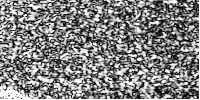
\includegraphics[width=0.5\linewidth]{example.png}
\caption{Selected picture.}
\label{fig:example}
\end{figure}






\section{Histogram}
\begin{lstlisting}[frame=tb]
 binwidth_complete <- 2*IQR(vexample$HH)*length(vexample$HH)^(-1/3)
 ggplot(data=vexample, aes(x=HH)) 
   geom_histogram(aes(y=..density..), 
                  binwidth = binwidth_complete)  
   xlab("Intensities") 
   ylab("Proportions") 
   ggtitle("Complete Histogram") 
   theme_few()
\end{lstlisting}
\begin{figure}
	\centering
	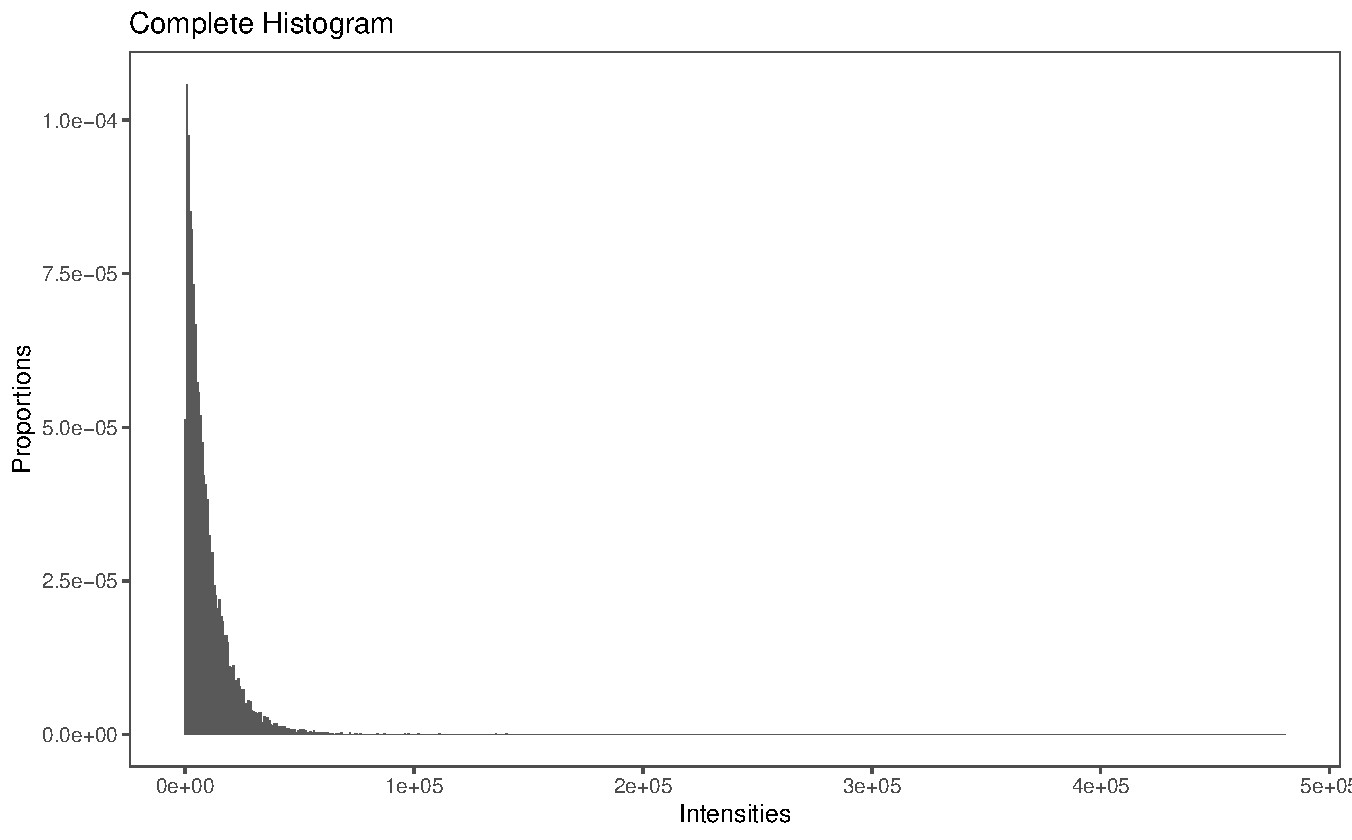
\includegraphics[width=0.5\linewidth]{HistogramExample.pdf}
	\caption{HistogramExample.}
	\label{fig:HistogramExample}
\end{figure}
\section{HistogramRestricted}
\begin{lstlisting}[frame=tb]
  ggplot(data=vexample, aes(x=HH)) 
  geom_histogram(aes(y=..density..), 
                 binwidth = binwidth_complete,
                 col="white")  
  xlab("Intensities") 
  xlim(0, 66666) 
  ylab("Proportions") 
  ggtitle("Restricted Histogram") 
  theme_few()
ggsave(filename = "./HistogramRestrictedExample.pdf")
\end{lstlisting}

\begin{figure}
	\centering
	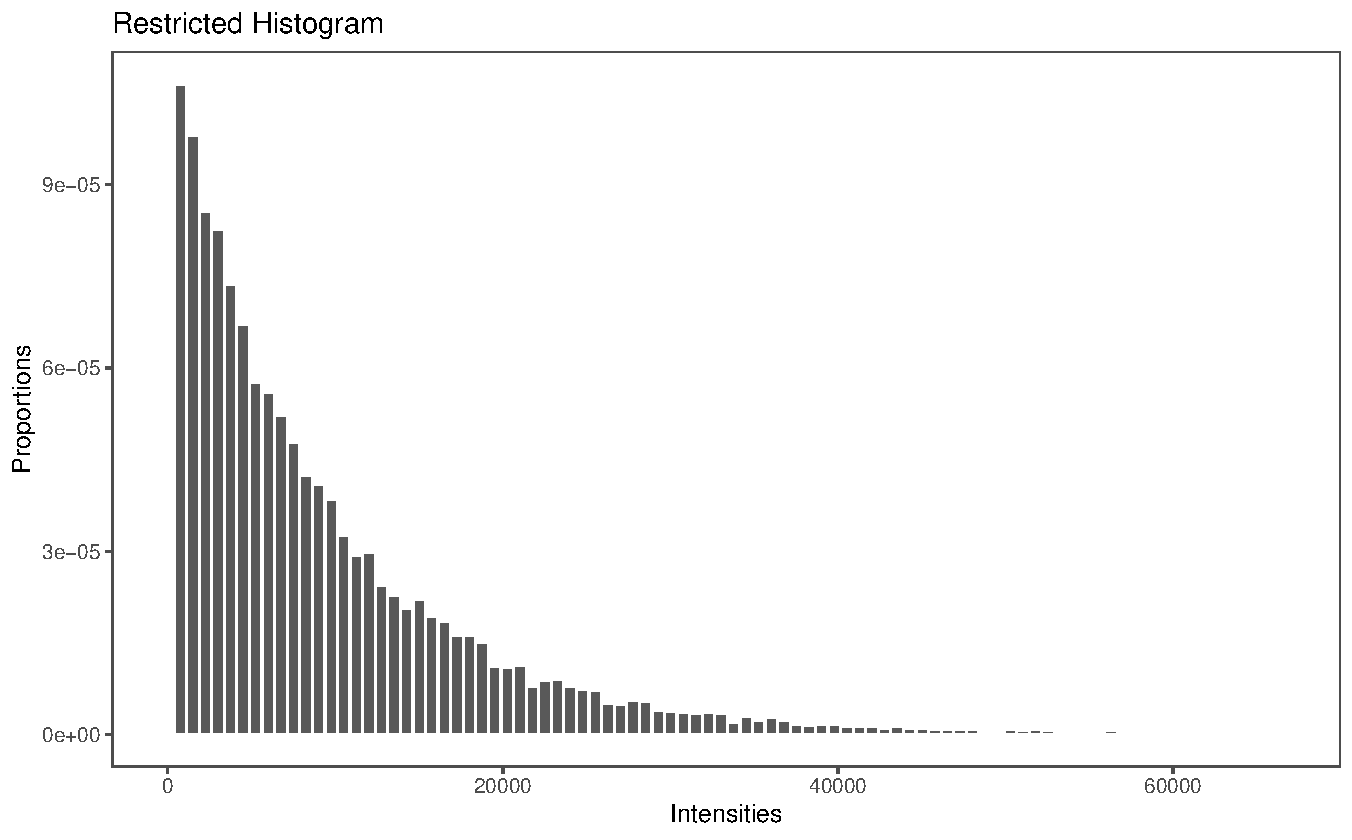
\includegraphics[width=0.5\linewidth]{HistogramRestrictedExample}
	\caption{HistogramRestricted.}
	\label{fig:HistogramExample}
\end{figure}

\section{LogLikelihood}
\begin{lstlisting}[frame=tb]
 LogLikelihoodLknown <- function(params) {
   
   p_alpha <- -abs(params[1])
   p_gamma <- abs(params[2])
   p_L <- abs(params[3])
   n <- length(z)
   return(
     n*(lgamma(p_L-p_alpha) - p_alpha*log(p_gamma) - lgamma(-p_alpha))  
       (p_alpha-p_L)*sum(log(p_gamma + z*p_L)) 
   )
 }
\end{lstlisting}
\section{Estimation}
\begin{lstlisting}[frame=tb]
 estim.exampleML <- maxNR(LogLikelihoodLknown, 
                        start=c(estim.example$alpha, estim.example$gamma,1), 
                        activePar=c(TRUE,TRUE,FALSE))$estimate[1:2]
 estim.exampleML
 -3.79  28101.39
\end{lstlisting}
results all above
\end{document}
